\begin{frame}
    \frametitle{The game}
    \centering
    
\includegraphics[scale=0.1]{Bin/cartoon_pics/ambulance_cartoon.png}

    \vspace{0.5cm}
    
\begin{tikzpicture}
        \draw[->, ultra thick] (-0.5, 0) -- ++(-1.5, -2);
        \draw[->, ultra thick] (0.5, 0) -- ++(1.5, -2);
    \end{tikzpicture}

    \vspace{0.5cm}
    
\includegraphics[scale=0.1]{Bin/cartoon_pics/hospital.png}
    \hspace{3cm}
    
\includegraphics[scale=0.1]{Bin/cartoon_pics/hospital.png}

\end{frame}


\begin{frame}
    \frametitle{Players - Strategies - Objectives}
    \centering

    
\includegraphics[scale=0.1]{Bin/cartoon_pics/ambulance_cartoon.png}
    \hspace{2cm}
    
\includegraphics[scale=0.1]{Bin/cartoon_pics/hospital.png}
    \hspace{2cm}
    
\includegraphics[scale=0.1]{Bin/cartoon_pics/hospital.png}

    \vspace{1cm}
    
\includegraphics[scale=0.2]{Bin/cartoon_pics/arrows.png}
    \hspace{2cm}
    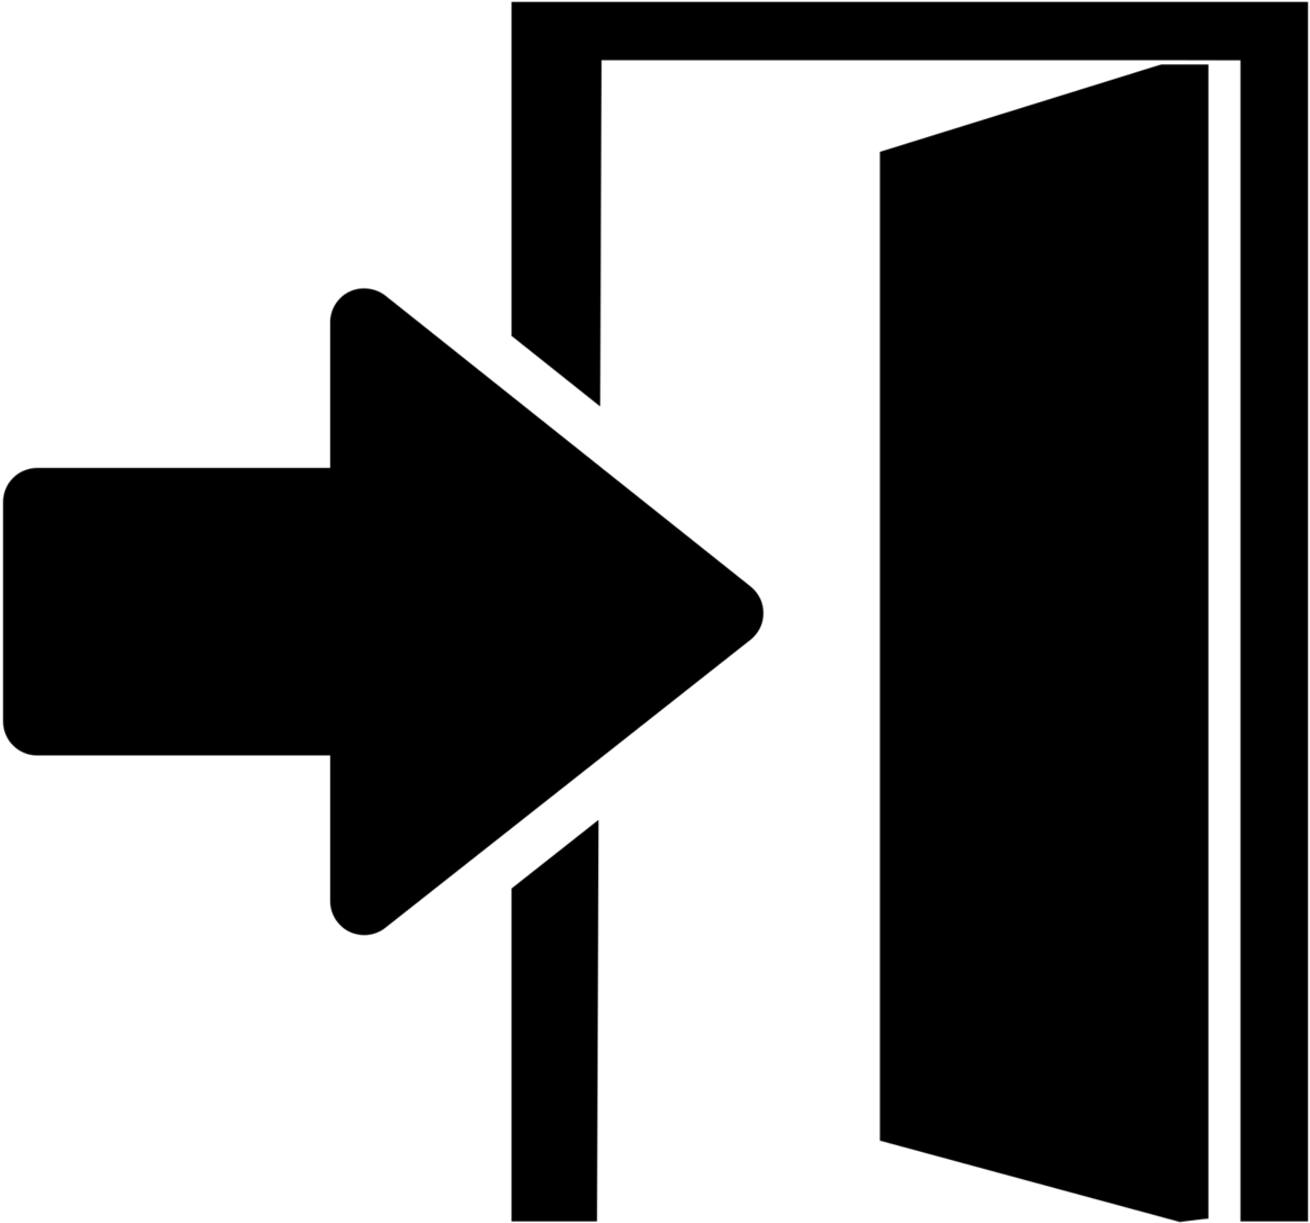
\includegraphics[scale=0.04]{Bin/cartoon_pics/door.png}
    \hspace{2cm}
    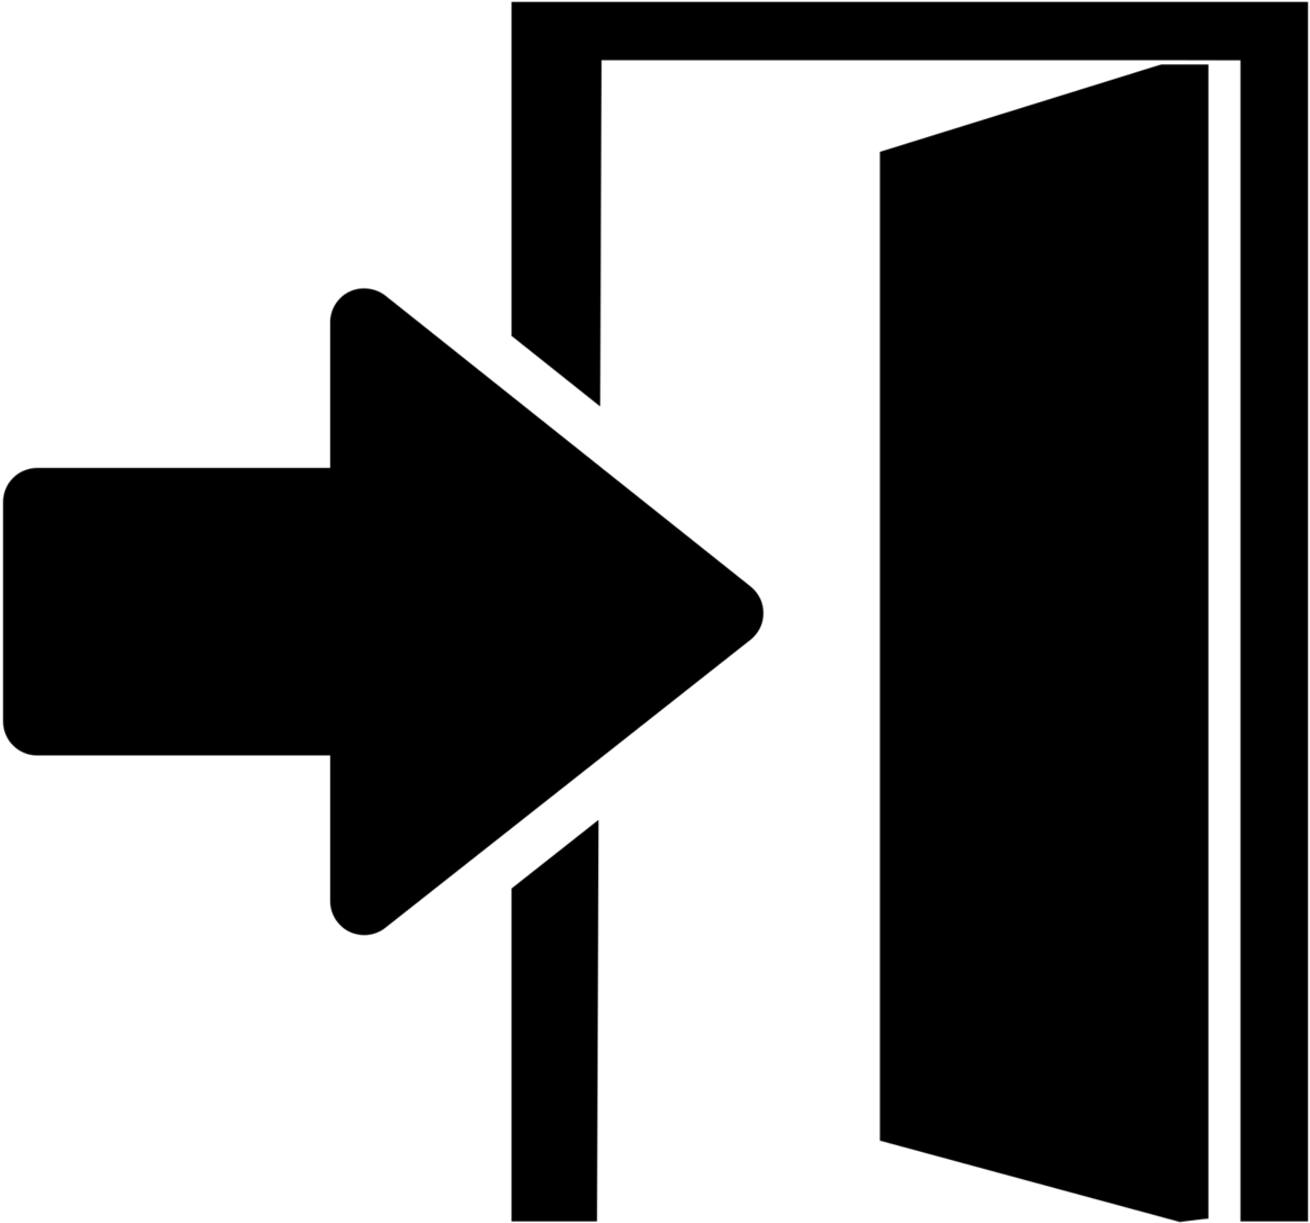
\includegraphics[scale=0.04]{Bin/cartoon_pics/door.png}

    \(p_A, p_B \in [0, 1] \hspace{2cm} T_A \in [1, N_A] 
    \hspace{2cm} T_B \in [1, N_B]\)    
    \(p_A + p_B = 1 \hspace{8cm}\)
    
    \vspace{1cm}
    \small
    \(
        \qquad \min \bar{B} \hspace{2.4cm} P(W^{(A)} < t) > 0.95 
        \hspace{0.7cm} P(W^{(B)} < t) > 0.95
    \)
\end{frame}


\begin{frame}
    \frametitle{Imperfect information extensive form game}
    \centering

    \begin{figure}[ht]
        \centering
        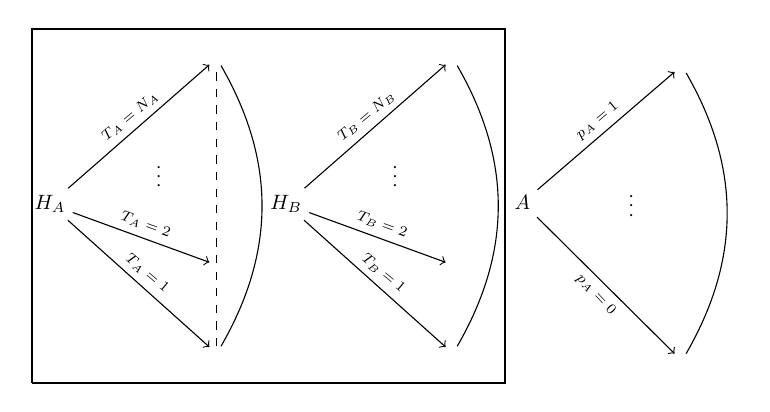
\begin{tikzpicture}[-, node distance = 2cm, scale=0.75, auto, rotate=90, transform shape]

            \only<2>{
                \draw[thick] (-3, 0) -- (3, 0) -- (3, -8) -- (-3, -8) -- (-3, 0);
            }

            \node[anchor=north, rotate=270] (QA) at (0.3,-0.3) {\(H_A\)};
            \node[anchor=north](QA_d1) at (-2.5, -3) {};
            \node[anchor=north](QA_d2) at (-1, -3) {};
            \node[anchor=north](QA_d3) at (0.5, -2) {\(\dots\)};
            \node[anchor=north](QA_d4) at (2.5, -3) {};
        
            \path[->] (QA) edge node [above, rotate=180+50] {\scriptsize{\(T_A=1\)}}(QA_d1);
            \path[->] (QA) edge node [above, rotate=180+70] {\scriptsize{\(T_A=2\)}}(QA_d2);
            \path[<-] (QA_d4) edge node [above, rotate=310] {\scriptsize{\(T_A = N_A\)}}(QA);
        
            \path (QA_d1) [dashed] edge node {}(QA_d4);
            \path (QA_d1) [bend right] edge node {}(QA_d4);
        
            \node[anchor=north, rotate=270](QB) at (0.3, -4.3) {\(H_B\)};
            \node[anchor=north](QB_d1) at (-2.5, -7) {};
            \node[anchor=north](QB_d2) at (-1, -7) {};
            \node[anchor=north](QB_d3) at (0.5, -6) {\(\dots\)};
            \node[anchor=north](QB_d4) at (2.5, -7) {};
        
            \path[->] (QB) edge node [above, rotate=180+50] {\scriptsize{\(T_B=1\)}}(QB_d1);
            \path[->] (QB) edge node [above, rotate=180+70] {\scriptsize{\(T_B=2\)}}(QB_d2);
            \path[<-] (QB_d4) edge node [above, rotate=310] {\scriptsize{\(T_B = N_B\)}}(QB);
        
            \path (QB_d1) [bend right] edge node {}(QB_d4);
        
            \node[anchor=north, rotate=270] (D) at (0.3, -8.3) {\(A\)};
            \node[anchor=north, rotate=270](D_d1) at (-2.5, -11) {};
            \node[anchor=north](D_dots) at (0, -10) {\(\dots\)};
            \node[anchor=north, rotate=270](D_d2) at (2.5, -11) {};
        
            \path[->] (D) edge node [below, rotate=180+43] {\scriptsize{\(p_A=0\)}}(D_d1);
            \path[<-] (D_d2) edge node [above, rotate=310] {\scriptsize{\(p_A=1\)}}(D);
        
            \path (D_d1) [bend right] edge node {}(D_d2);
        
        \end{tikzpicture}        
    \end{figure}
\end{frame}